%& preamble - kommer användas i subfiles med
\documentclass{article}
\usepackage[utf8]{inputenc}
\usepackage[swedish]{babel}
\usepackage{parskip}
\usepackage{pgffor}
\usepackage{amsmath}
\usepackage{tikz}
\usepackage{tkz-euclide}
\usepackage{pdfpages}
\usepackage{hyperref}
\usepackage{xcolor}
\usepackage{graphicx}

% lägg till egna macros
% för att enkelt formattera lösningar
\newenvironment{solution}[1]
    {\addcontentsline{toc}{subsubsection}{#1}{\Large\textbf{#1.}}\newline}
    {\newline}

\newcommand{\subsolution}[1]{{\large\textbf{#1)}\newline}}

% för att skapa "formler"
\newtheorem{formel}{Formel}

% kommando för att skriva R^n
\newcommand{\Rn}[1]{\mathbb{R}^{#1}}

% environment för att enkelt skapa rutnät där man kan rita vektorer
\newenvironment{vectors2d}[4]
{
\begin{center}
\begin{tikzpicture}[scale=0.5]
  \draw[thin,gray!40] (#1,#2) grid (#3,#4);
  \draw[<->] (#1,0)--(#3,0) node[right]{$x$};
  \draw[<->] (0,#2)--(0,#4) node[above]{$y$};
}
{
\end{tikzpicture}
\end{center}
}
% Lägg in sånna här för att rita vektorer:
% \draw[line width=1pt,gray!40,-stealth](2,3)--(1,-2) node[anchor=south west]{$\vec{u}$};
% om man vill färga den:
% \draw[line width=1pt,blue,-stealth](2,3)--(1,-2) node[anchor=south west]{$\vec{u}$};


%% inkludera alla lösningar i en mapp 
%% uppgifter som saknas skrivs upp i table of contents med, fast som missing
\newcommand{\inkluderauppgifter}[2]{
\foreach \i in {1, ..., #2} {
    \edef\FileName{#1/\i}%
    \IfFileExists{\FileName}{%
       \subfile{\FileName}%
    }{%else
        {\addcontentsline{toc}{subsubsection}{\color{red} \i - lösning saknas}}%
    }%
}%
}




%% totalmatris
% https://tex.stackexchange.com/questions/2233/whats-the-best-way-make-an-augmented-coefficient-matrix
\makeatletter
\renewcommand*\env@matrix[1][*\c@MaxMatrixCols c]{%
  \hskip -\arraycolsep
  \let\@ifnextchar\new@ifnextchar
  \array{#1}}
\makeatother

\usepackage{subfiles} % inkluderar allt innan i subfiles, så bör komma sist.


\title{SF1624 - Algebra och geometri\\ {\large detaljerade lösningar till rekommenderade uppgifter}\\
\bigskip
\includegraphics[scale=0.25]{qrcode.png}\\
{\small work in progress, hämta senaste versionen på}
\\ {\small \url{https://github.com/simon-rosen/linalg-2022/blob/main/linalg_2022.pdf}}}


\begin{document}

\maketitle

\newpage 

\tableofcontents

\newpage

\section{modul 1}
%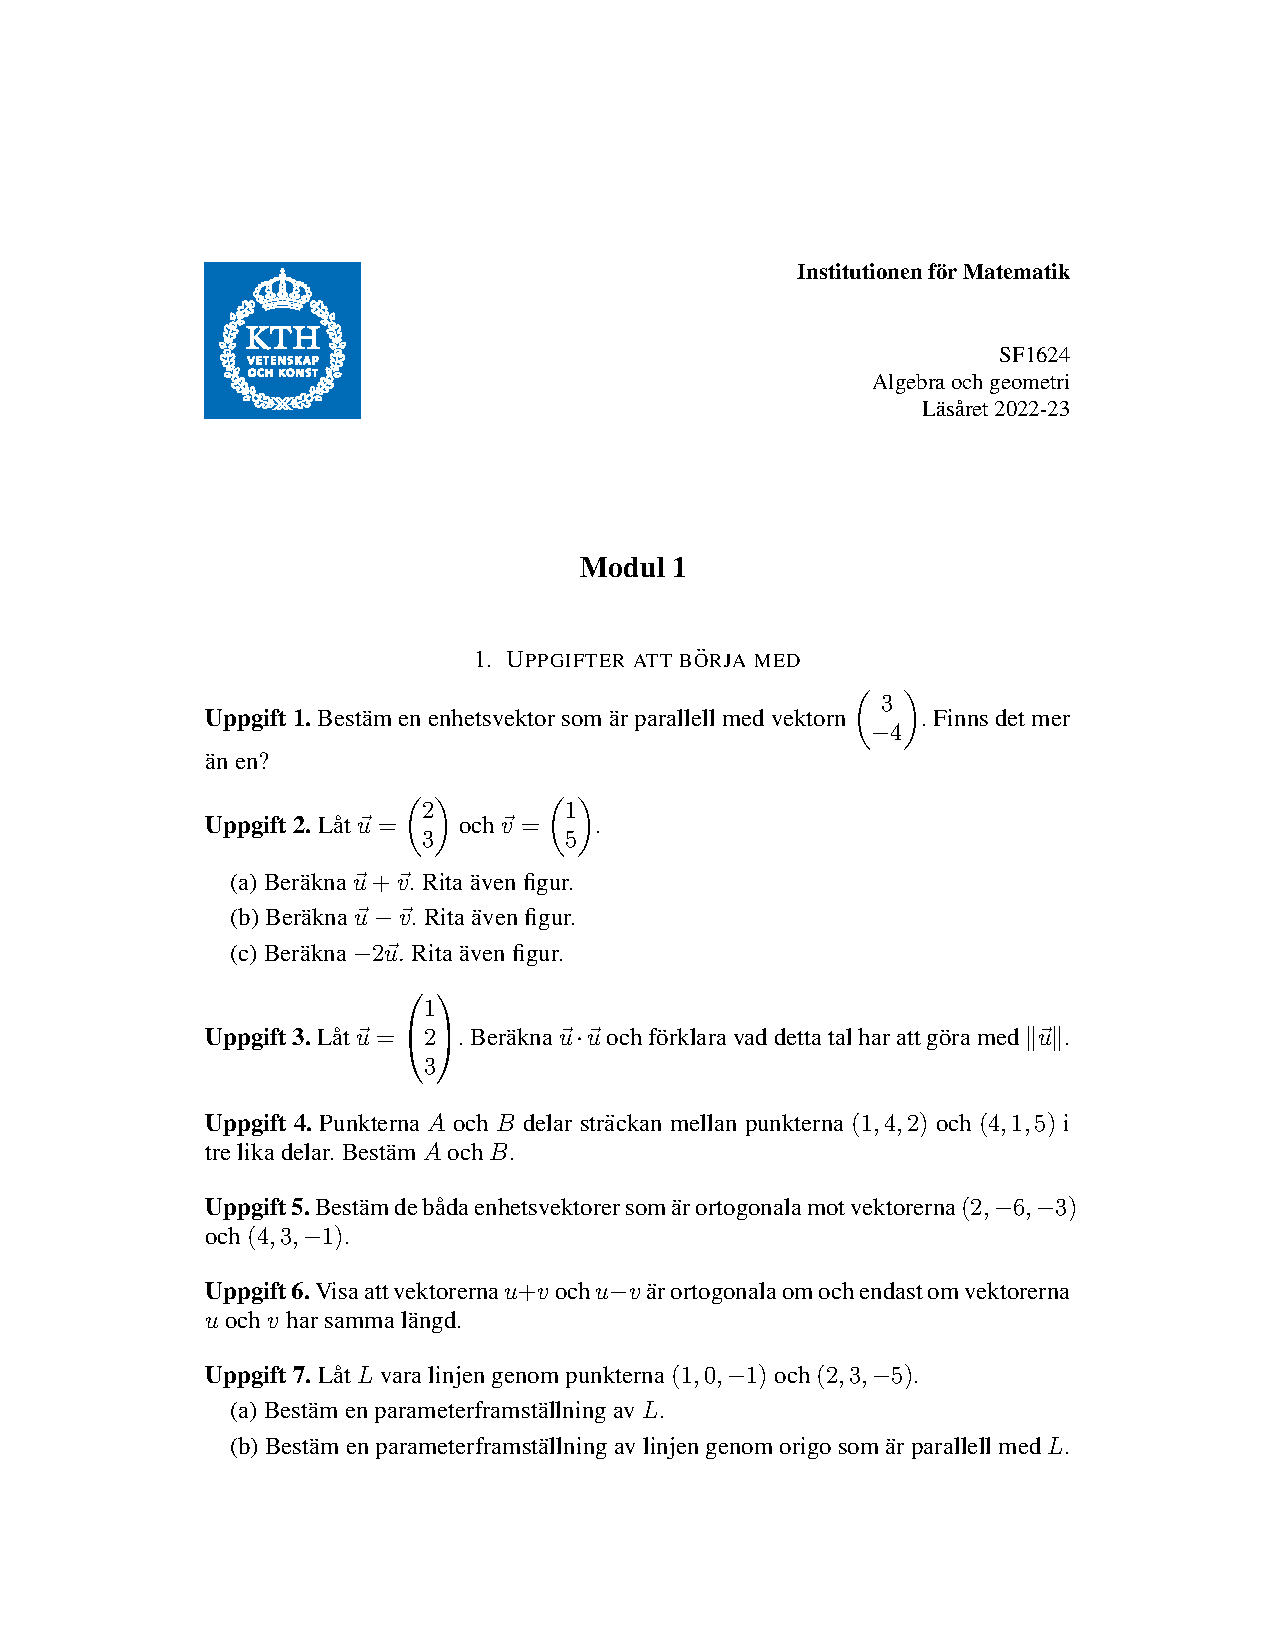
\includepdf[pages=-]{pdfs/22Modul1.pdf} % ska nog inte vara med i slutgiltig version, men nice att ha när man löser uppgifterna


\subsection{Teori}
\subfile{modul1/teori}

\subsection{Uppgifter att börja med}
\inkluderauppgifter{modul1/uppgifter_att_borja_med}{26}


\section{modul 2}
%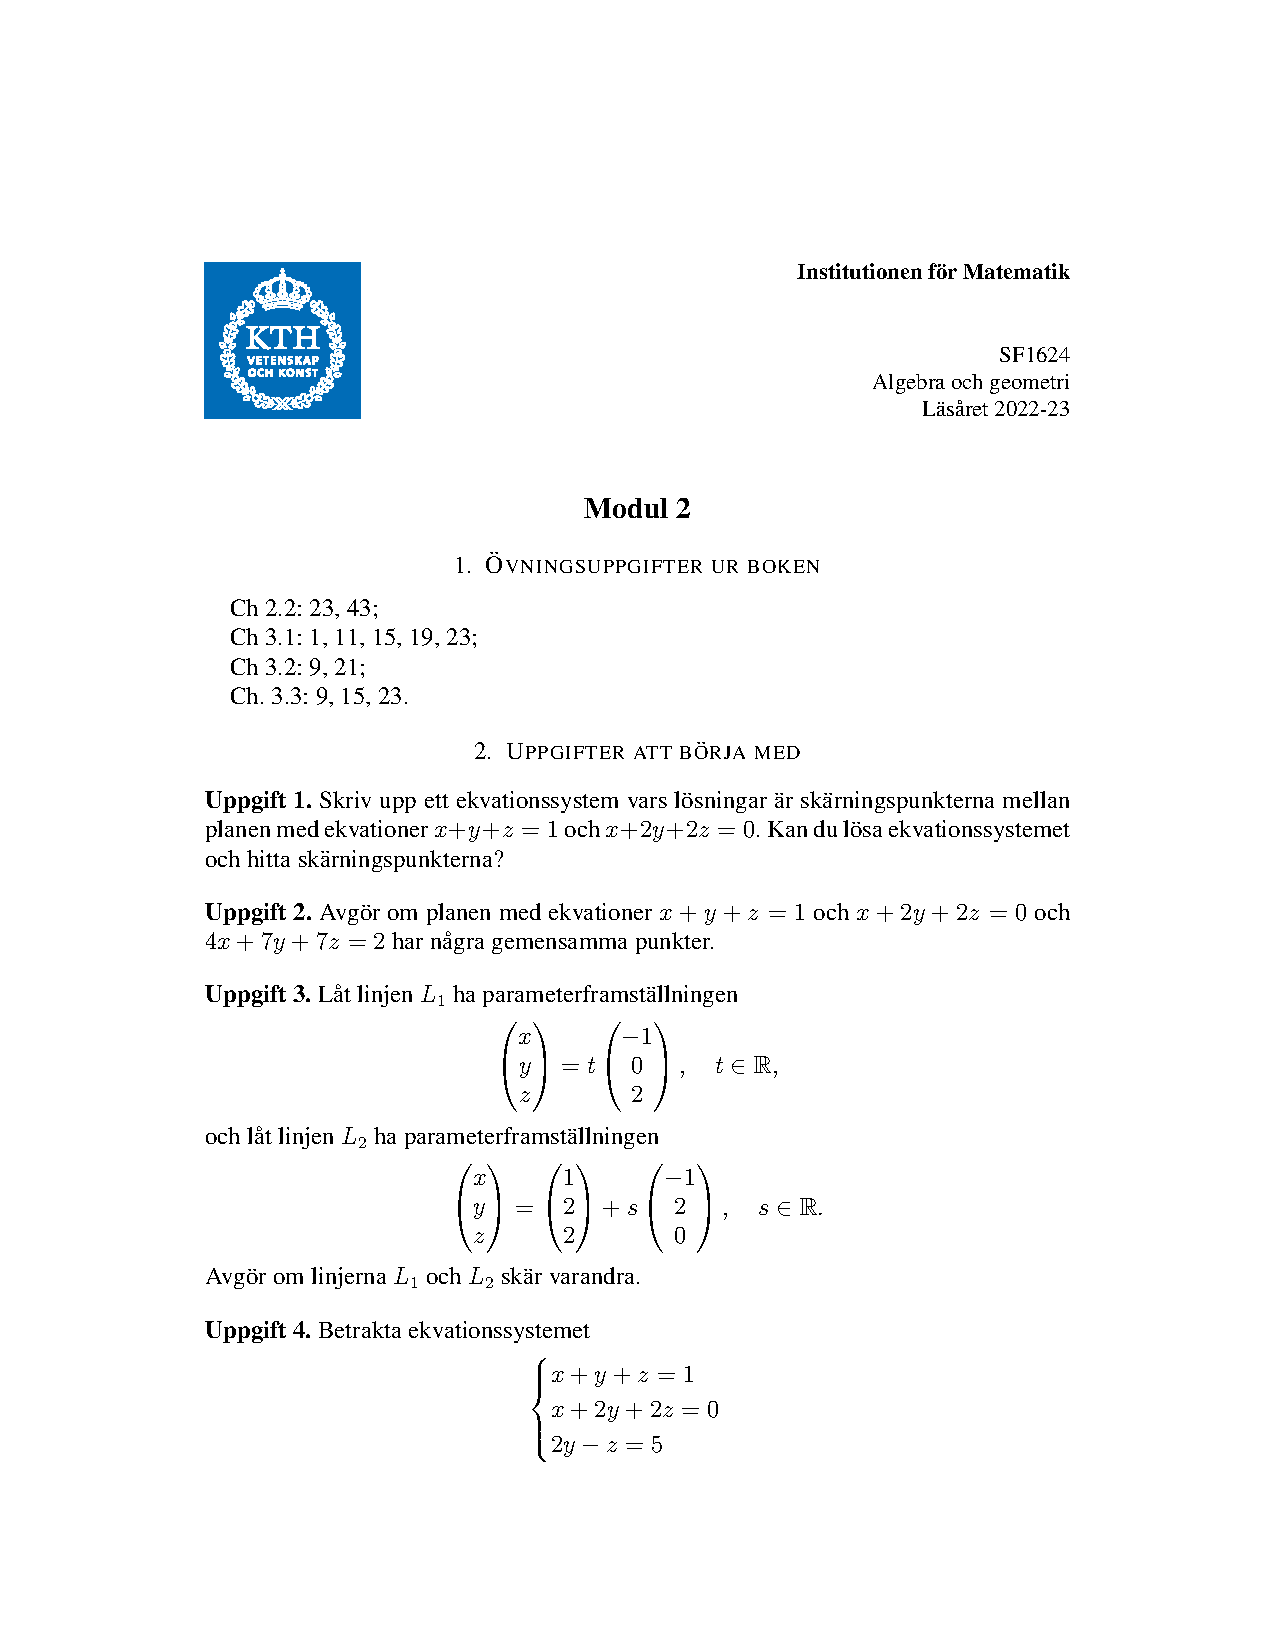
\includepdf[pages=-]{pdfs/22Modul2.pdf} % ska nog inte vara med i slutgiltig version, men nice att ha när man löser uppgifterna
\subsection{Teori}
\subfile{modul2/teori}

\subsection{Uppgifter att börja med}
\inkluderauppgifter{modul2/uppgifter_att_borja_med}{22}


\section{modul 3}
%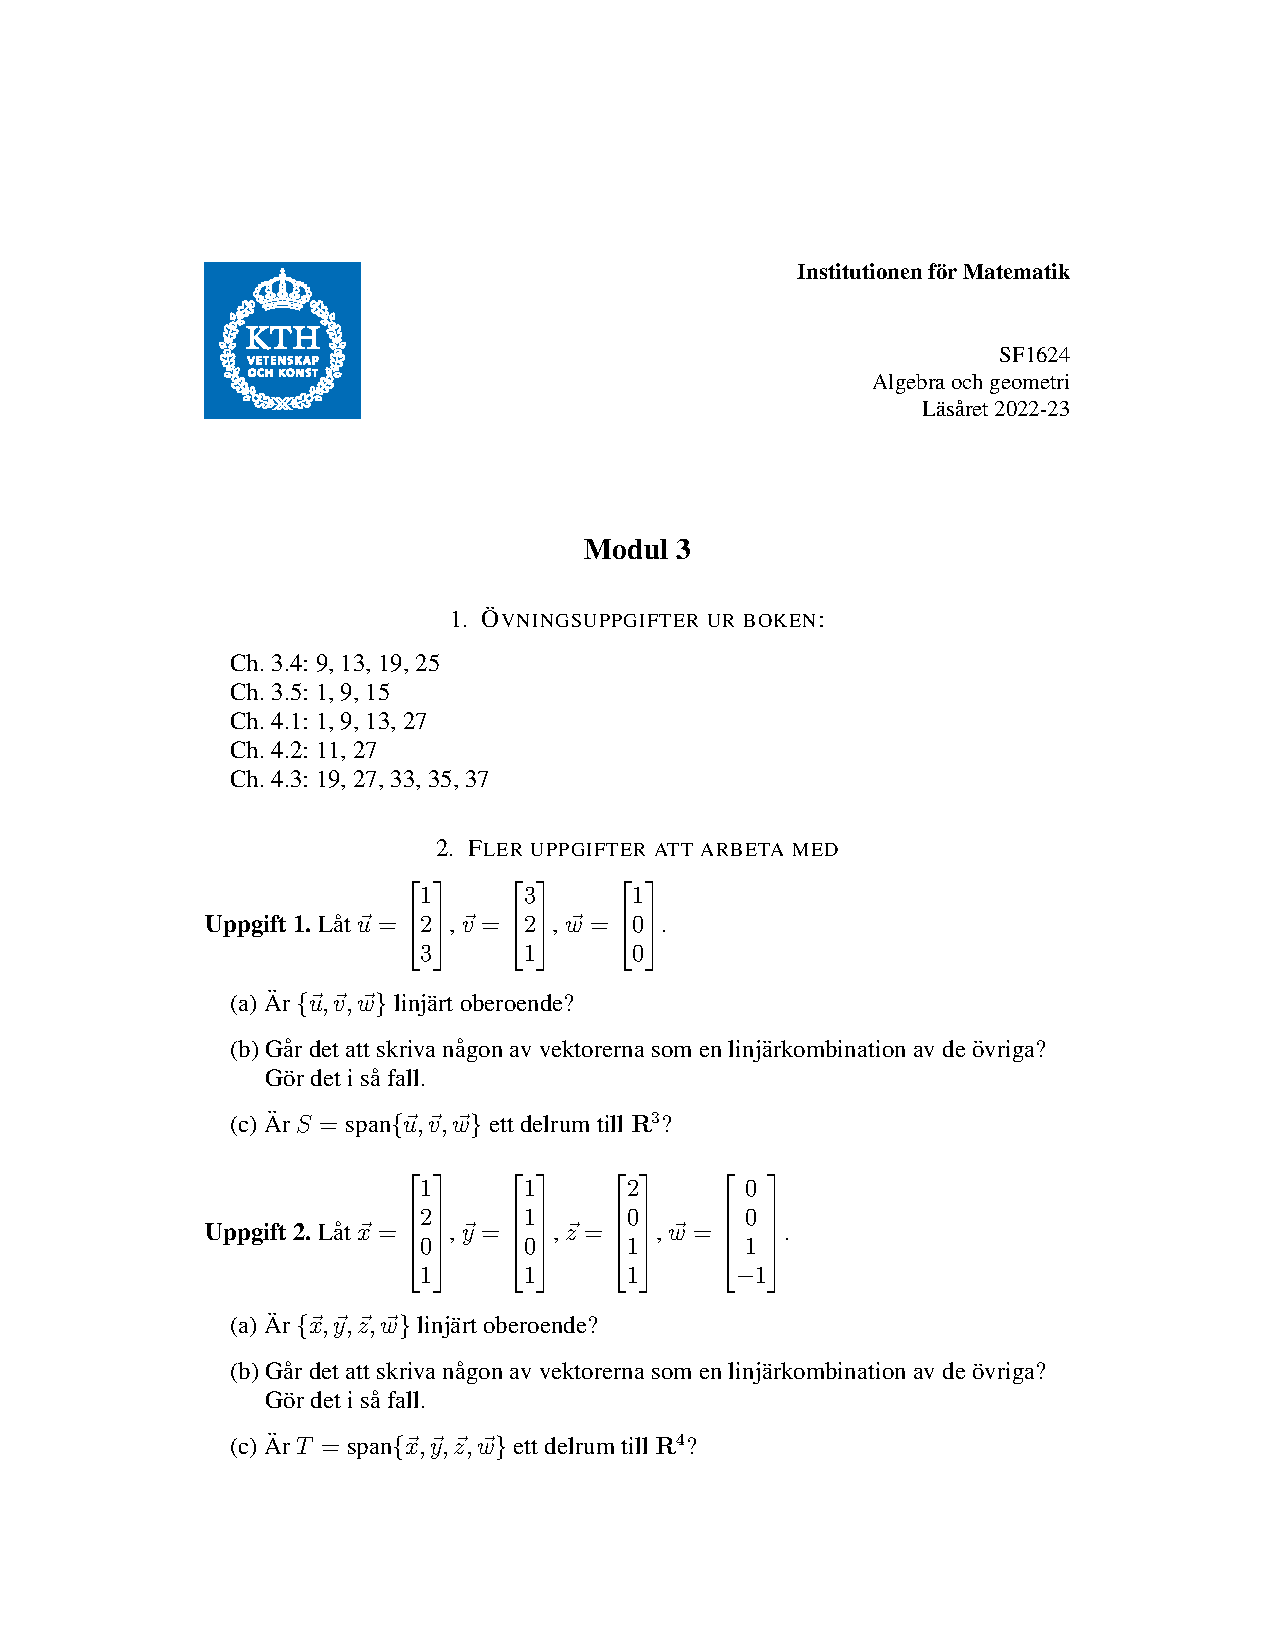
\includepdf[pages=-]{pdfs/22Modul3.pdf} % ska nog inte vara med i slutgiltig version, men nice att ha när man löser uppgifterna
\subsection{Teori}
\subfile{modul3/teori}

\subsection{Uppgifter att börja med}
\inkluderauppgifter{modul3/uppgifter_att_borja_med}{19}


\section{modul 4}
%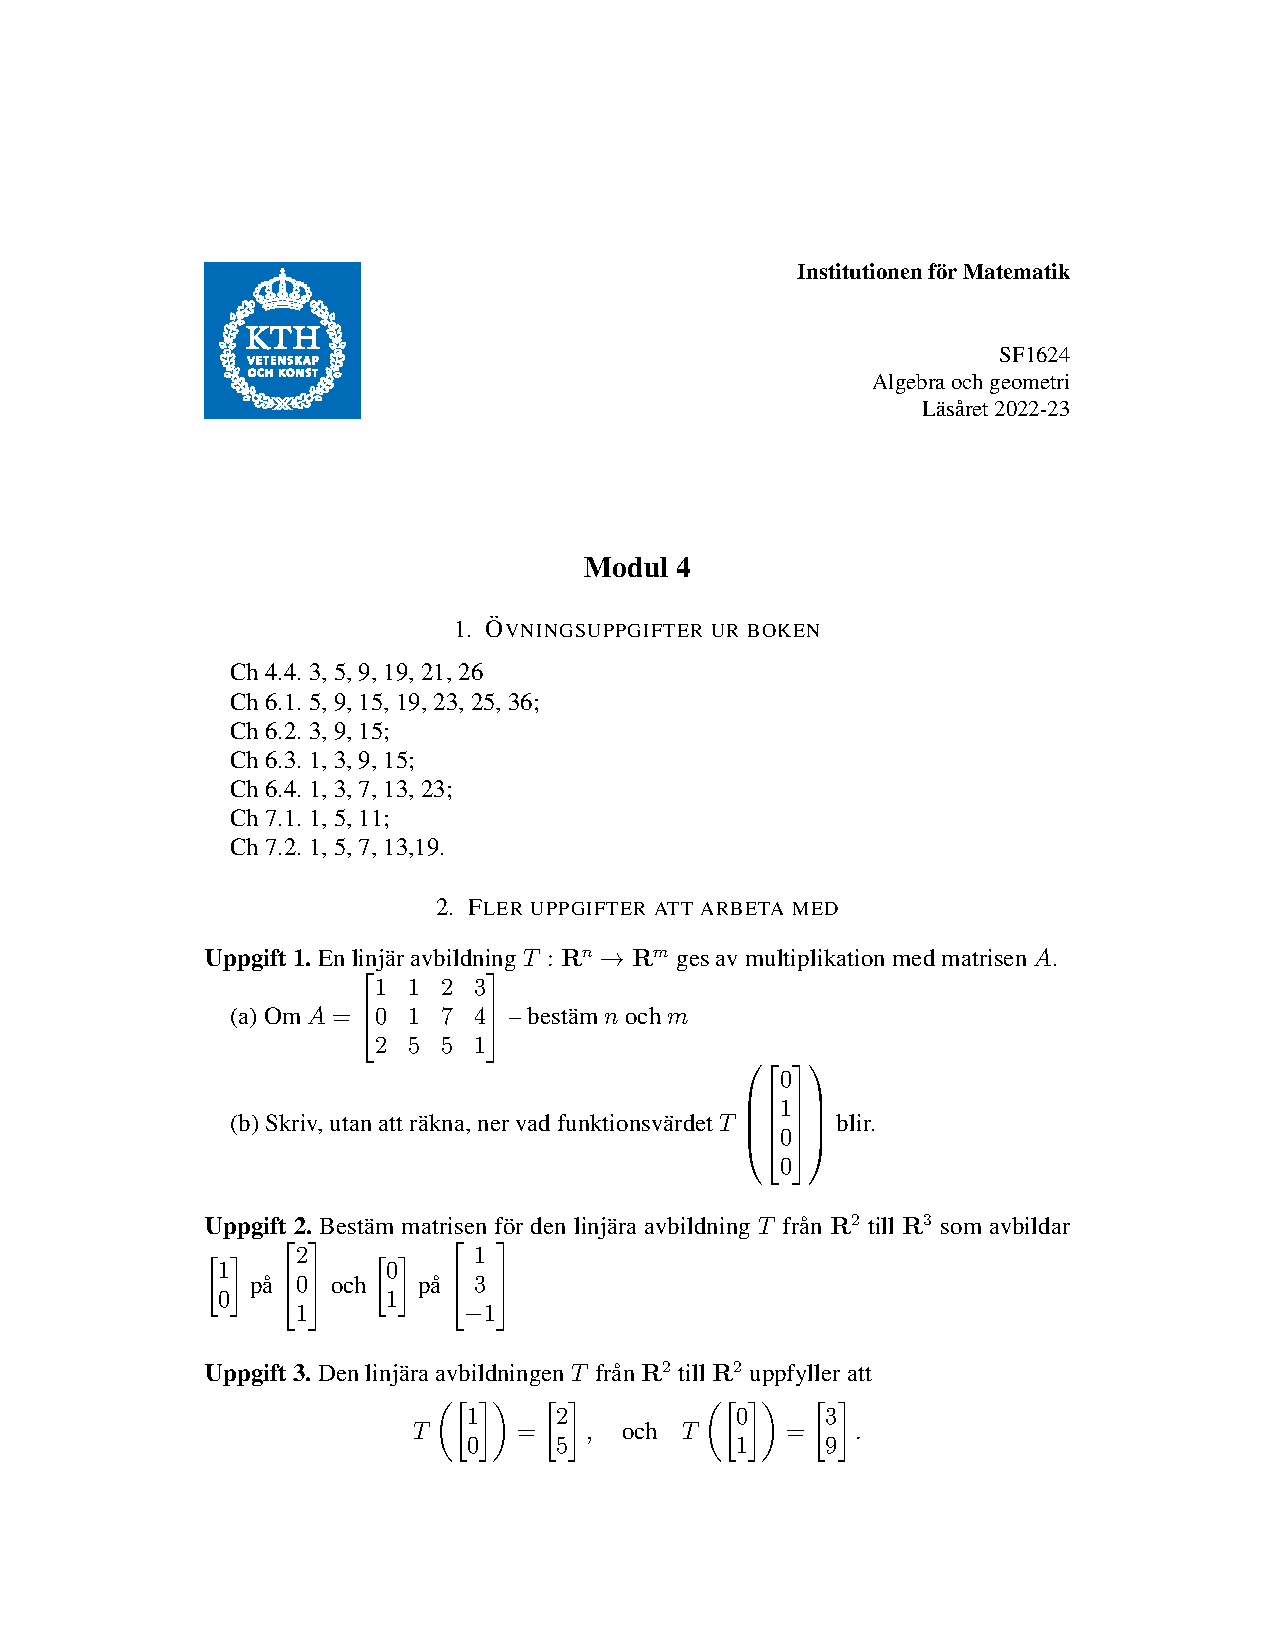
\includepdf[pages=-]{pdfs/22Modul4.pdf} % ska nog inte vara med i slutgiltig version, men nice att ha när man löser uppgifterna
\subsection{Teori}
\subfile{modul4/teori}

\subsection{Uppgifter att börja med}
\inkluderauppgifter{modul4/uppgifter_att_borja_med}{21}


\section{modul 5}
%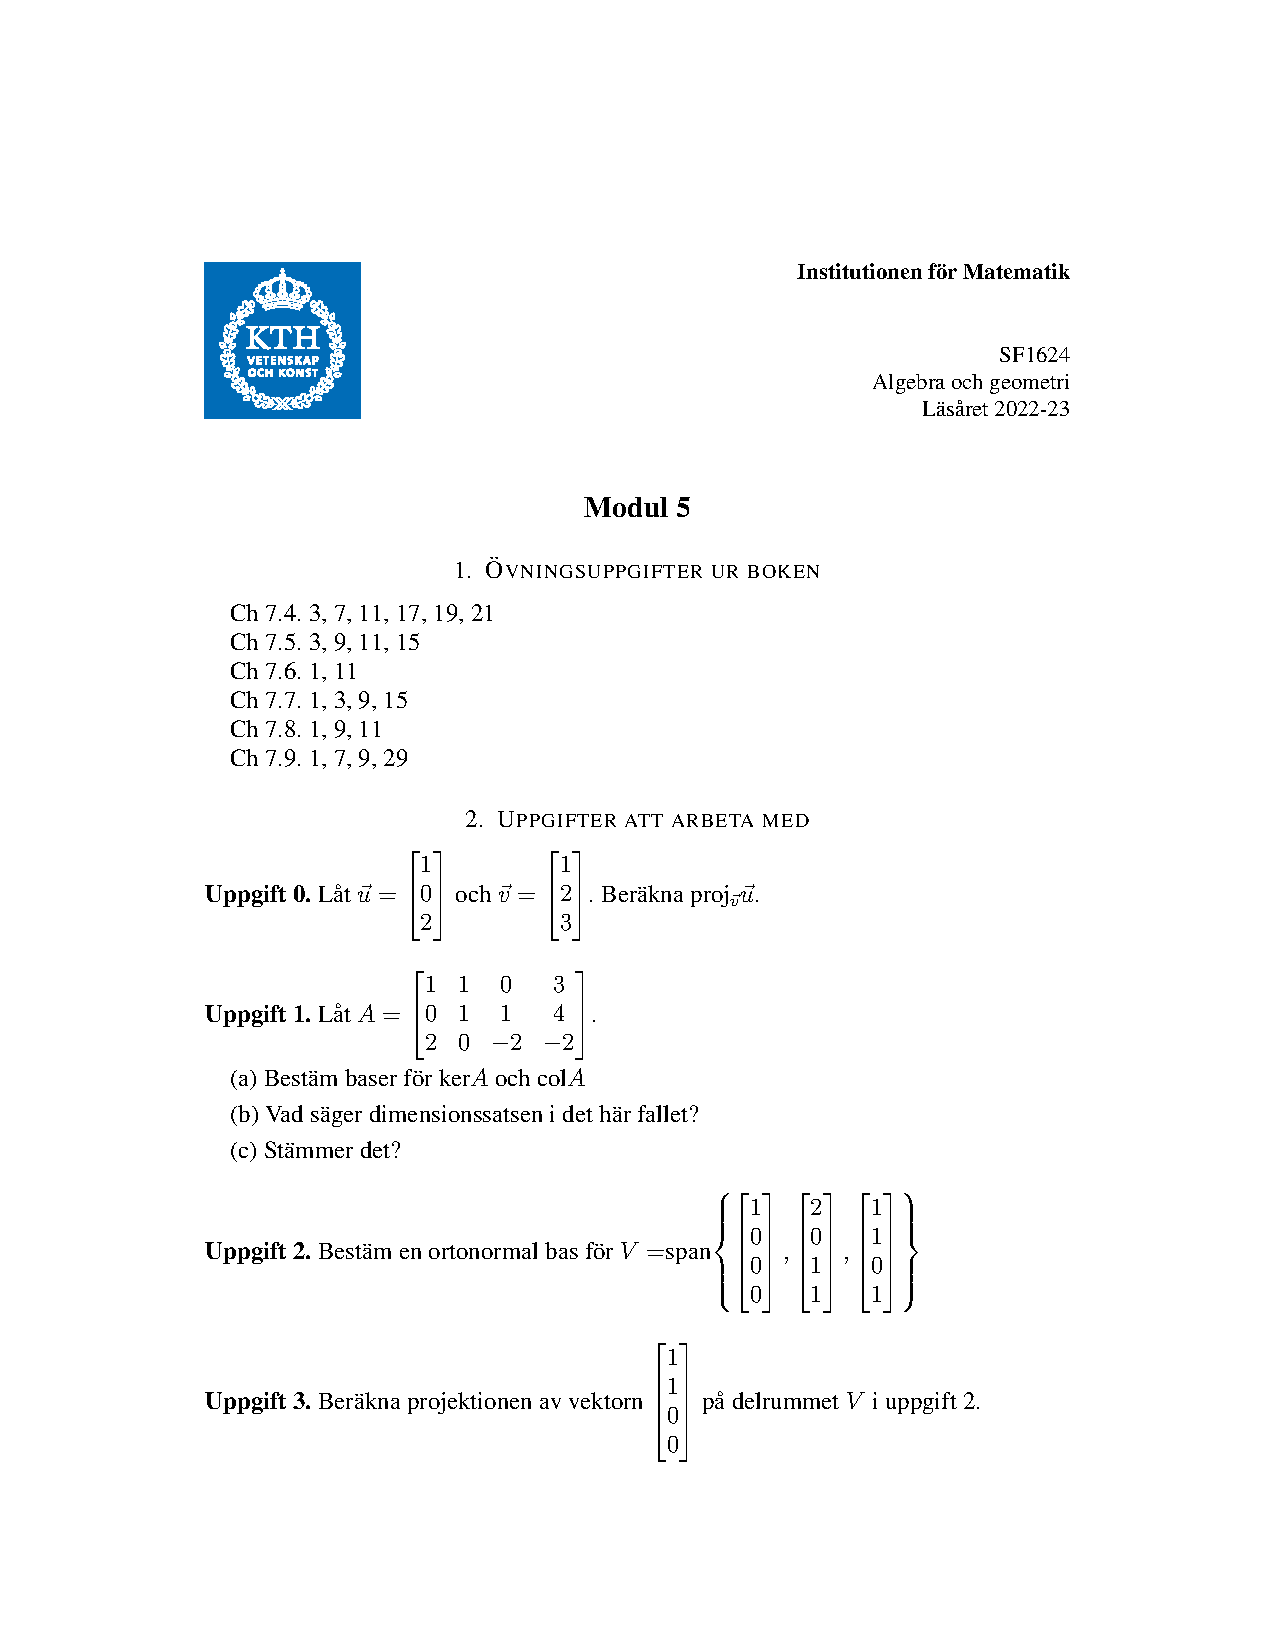
\includepdf[pages=-]{pdfs/22Modul5.pdf} % ska nog inte vara med i slutgiltig version, men nice att ha när man löser uppgifterna
\subsection{Teori}
\subfile{modul5/teori}

\subsection{Uppgifter att börja med}
\inkluderauppgifter{modul5/uppgifter_att_borja_med}{15}


\section{modul 6}
%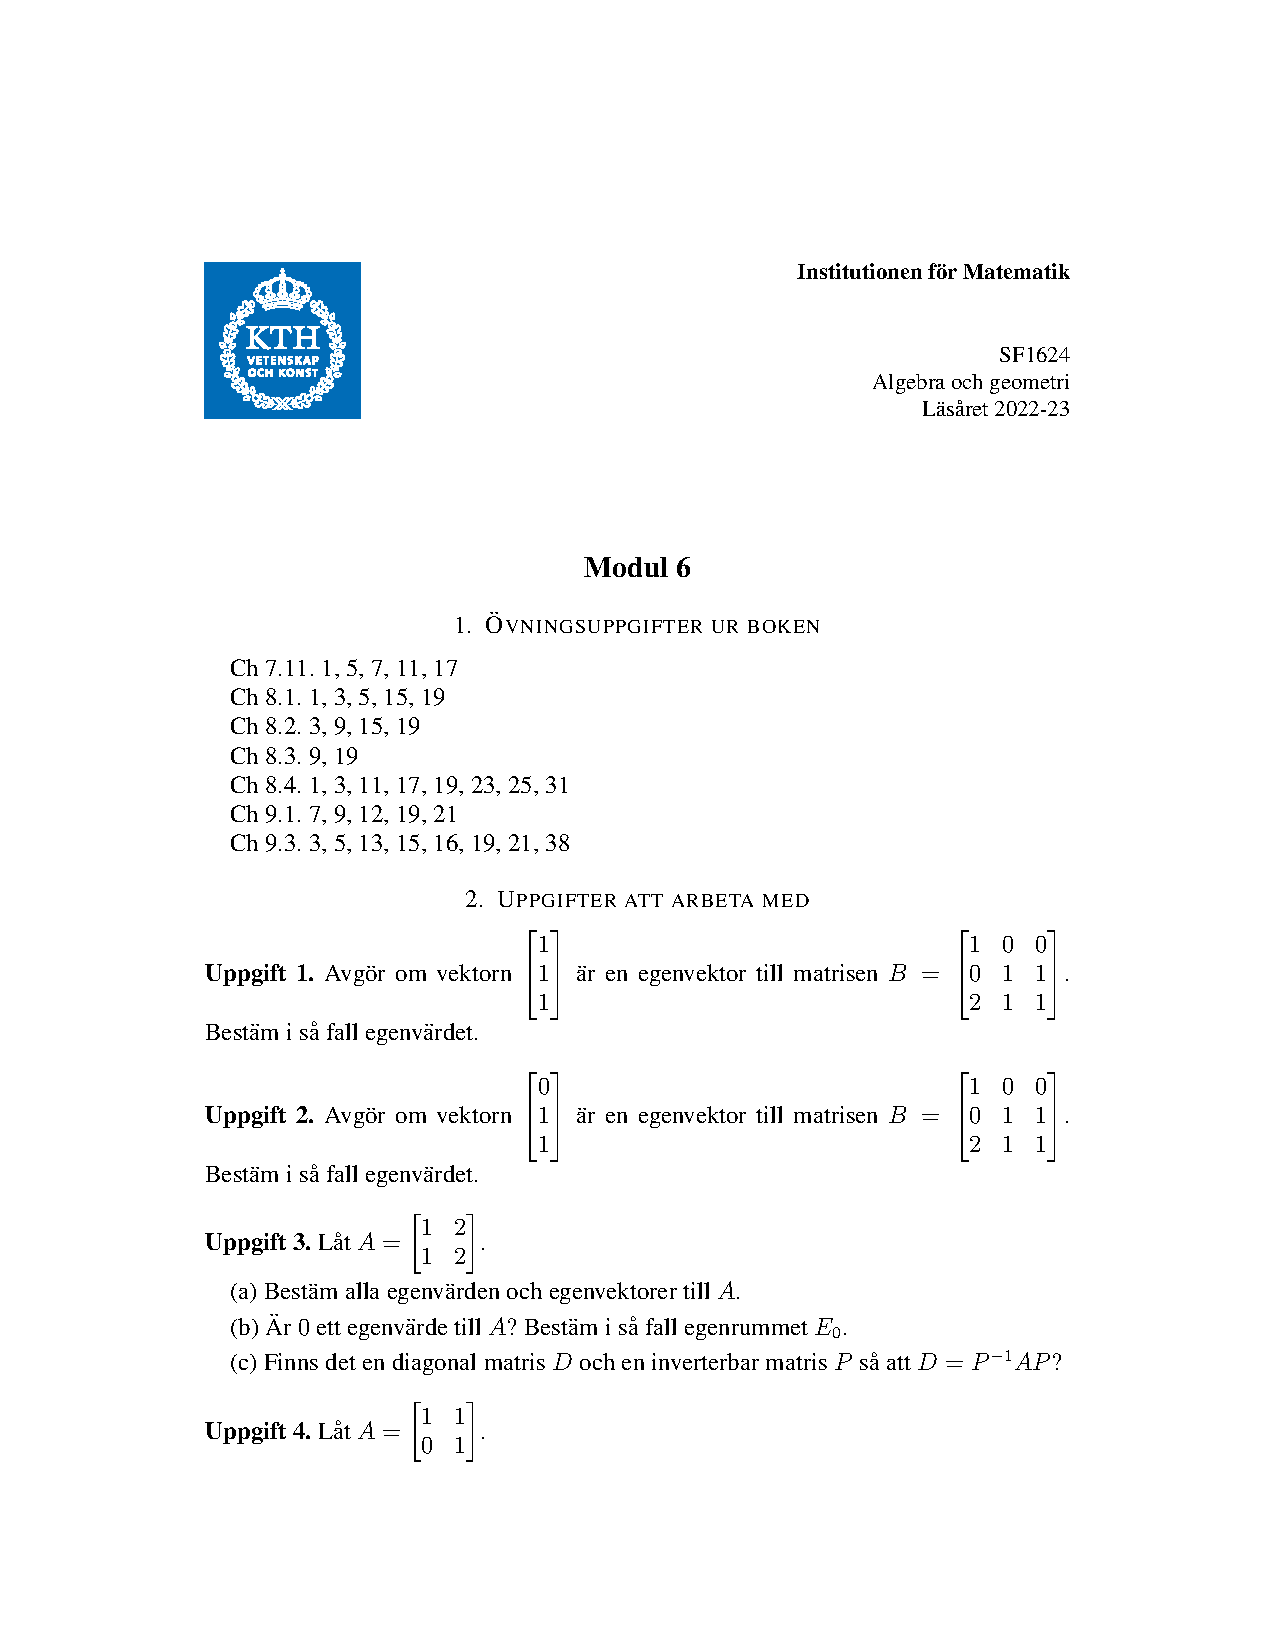
\includepdf[pages=-]{pdfs/22Modul6.pdf} % ska nog inte vara med i slutgiltig version, men nice att ha när man löser uppgifterna
\subsection{Teori}
\subfile{modul6/teori}

\subsection{Uppgifter att börja med}
\inkluderauppgifter{modul6/uppgifter_att_borja_med}{19}


\end{document}
